\chapter{Analiza problemu}
\thispagestyle{chapterBeginStyle}
\label{rozdzial1}

W niniejszym rozdziale zostanie zdefiniowany problem replikacji obrazów rozważany w pracy. Przedstawiona zostanie również koncepcja i założenia algorytmów stosowanych przez autora do testowania oraz praktycznego zobrazowania analizowanego problemu. Zostaną również omówione podstawowe pojęcie niezbędne do zrozumienia idei i genezy algorytmów metaheurystycznych.

\section{Replikacja obrazów}
 
Replikacją obrazów można określić proces, podczas którego oryginalny (wzorcowy) obraz jest reprodukowany za pomocą pewnej techniki. Użyto tutaj nie bez powodu słowa \textit{technika}, ponieważ, pomimo że praca skupia się na pewnym algorytmie i jego implementacji w wysokopoziomowym języku programowania, to sam proces replikacji (reprodukcji) nie jest pojęciem nowym. Stosowany on był już przez wiele stuleci w przeszłości przez artystów (malarzy, rzeźbiarzy), którzy zajmowali się kopiowaniem innych dział malarskich lub rzeźbiarskich. Idea przyświecająca osobom, kopiującym działa malarskie, w dobie obecnej technologii, została przeniesiona na grunt techniki cyfrowej. Obecnie istnieje wiele narzędzi (programów lub bibliotek współpracujących z językami programowania) umożliwiających wykonywanie operacji na cyfrowych formatach obrazów. Narzędzia te stosują pewne wyspecjalizowane algorytmy, gdzie zadaniem każdego z nich jest dokonanie na obrazie pewnych zmian. Wraz z rozwojem techniki cyfrowego przetwarzania obrazów, naturalnym jest, że zdecydowano się również na cyfrową reprodukcję.

W tym miejscu należy również zaznaczyć, że przedstawiany w pracy proces replikacji, do którego autor użył algorytmów genetycznych, nie polega na skopiowaniu pewnego obrazu w formie \textit{jeden do jednego}. Opisywany proces ma na celu jedynie przybliżenie danego obrazu, więc należy też rozpatrywać ten opisywany sposób jako formę procesu twórczego. Nie da się bowiem powiedzieć, że zawsze, po zakończeniu działania algorytmu otrzymane zostanie dokładnie to, co było kopiowane, to jest każdy piksel wyprodukowanego rozwiązania będzie identyczny jak piksel obrazu oryginalnego (rozumie się tutaj obraz przez pewną prostokątną macierz pikseli, gdzie każdemu pikselowi przyporządkowane są pewne wartości liczbowe określające jego barwę). Zamierzonym efektem jest to, że po zakończeniu działania algorytmu jest uzyskiwane jest jedynie pewien obraz podobny \footnote{\textit{Podobny} należy rozumieć jako obraz podobny pod względem wizualnym lub względem określonej funkcji mierzącej podobieństwo dwóch obrazów.} do swojego pierwowzoru i nie da się określić przed rozpoczęciem działania programu jaki wynik zostanie uzyskany.

\subsection{Idea cyfrowej replikacji obrazów}
\label{subsec:idea_of_dip}
Rozważając cyfrowe podejście do replikacji obrazów należy rozumieć ten proces jako zastosowanie pewnego algorytmu, który mając do dyspozycji obraz oryginalny (reprodukowany) dąży do tego, aby stworzyć jego jak najwierniejszą kopię lub, głównie w przypadku algorytmów uczenia maszynowego (ang. \textit{machine learning}), na podstawie pewnego zbioru obrazów utworzyć obraz mający cechy zbioru, na którym algorytm się uczył i jak najbardziej przypominający obraz stworzony przez człowieka (zdjęcie, rysunek, obraz namalowany przez malarza). Do tego celu wykorzystywane są sieci neuronowe, tzw. GANy (ang. \textit{Generative Adversarial Network}) mające swoje powszechne zastosowanie w \textit{deep learningu} (cf. \cite{GANS}).

\section{Cyfrowa reprezentacja obrazów}

Obraz w postaci cyfrowej jest reprezentowany na poziomie pamięci jako pewien ciąg bitów, jak wszystkie dane cyfrowe. Na poziomie języka programowania, w którym wykonywane są operacje na obrazie, obraz reprezentowany jest w pewnej skali kolorystycznej, np. RGBA, CMYK, HSV, CIELAB lub w skali szarości. Obraz przedstawiany jest jako macierz prostokątna $m \times n$ pikseli, gdzie każdemu pikselowi jest przyporządkowany pewien kolor. W przypadku niniejszej pracy autor będzie używał dwóch skali, za pomocą których obrazy mogą być reprezentowane cyfrowo - RGBA oraz skali szarości.

\subsection{Skala RGBA}
\label{subsec:rgba}

W modelu przestrzeni barw RGBA (cf. \cite{RGBASpecification}) obraz jest reprezentowany jako tablica pikseli o wymiarach $n \times m$. Każdy piksel (reprezentowany za pomocą pewnej struktury lub obiektu) posiada informację o kolorze w tym przypadku zapisywaną za pomocą czterech parametrów zwanych kanałami. Pierwsze trzy kanały (RGB) reprezentują kanałowi czerwonemu (ang. \textit{red}), zielonemu (ang. \textit{green}) oraz niebieskiemu (ang. \textit{blue}). Ostatni kanał A jest nazywany kanałem \textit{alfa} i określa on stopień przeźroczystości danego piksela. Skala ta została schematycznie przedstawiona na rysunku \ref{fig:rgb_cube}. Każdy z wymiarów przedstawionego na grafice sześcianu reprezentuje jeden z kanałów RGB. Zakładając, że do reprezentacji używa się dodatnich liczb całkowitych 8-bitowych, wówczas każda ze ścian tego sześcianu ma wymiary $255 \times 255$. Każda współrzędna $(r, g, b)$ odpowiada konkretnemu kolorowi ze skali. Jest to jednak jedynie przedstawienie samej skali RGB. W celu uzyskania skali RGBA, na przedstawioną na grafice kostkę należy jeszcze nałożyć kanał \textit{alfa}. Wówczas z trójek uporządkowanych określających współrzędne otrzymuje czwartą wartość $\alpha$, która definiuje jej przeźroczystość, którą, w celu lepszego uzmysłowienia czytelnikowi czym jest $\alpha$, można nazwać \textit{widocznością} danego koloru.

Skala RGBA jest stosowana m. in. w formacie \texttt{PNG} służącym do zapisu grafiki oraz jest powszechnie stosowana w programach do obróbki graficznej oraz w bibliotekach języków programowania służących do przetwarzania zdjęć.

\begin{figure}
    \centering
    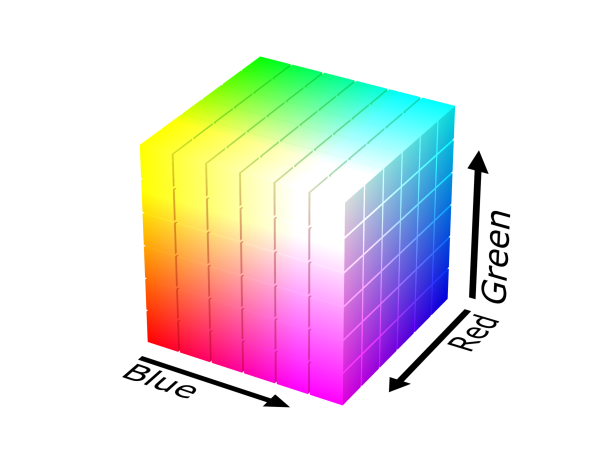
\includegraphics[scale=1.8]{images/other/RGB_color_small.png}
    \caption{
        Schematyczne przedstawienie skali RGB. Każdy voxel sześcianu reprezentuje unikalny kolor. Można zatem każdy kolor zapisać za pomocą trójki uporządkowanej $(R, G, B)$, aby wskazać konkretny odcień. \\ 
        (\textit{Żródło:} \cite{RGBCube})
    }
    \label{fig:rgb_cube}
\end{figure}

\subsection{Skala szarości}

W skali szarości, w przeciwieństwie do opisywanej w podrozdziale \ref{subsec:rgba} skali RGBA, rozważa się tylko jeden kanał. Określa on jedynie intensywność danego piksela. W przypadku, gdy ten kanał reprezentowany jest przez 8-bitowe dodatnie liczby całkowite, wówczas wartość 0 oznacza najmniejszą intensywność (reprezentowany jako kolor czarny), a wartośc maksymalna 255 oznacza największą intensywność (reprezentowaną jako kolor biały).

Skala szarości jest również podzbiorem skali RGBA - rozważane są w niej takie kolory, w których pierwsze trzy kanały (RGB) maja dokładnie taką samą wartość. Dla skali szarości nie rozważa się wówczas kanału \textit{alfa} i przyjmuje się, że zawsze przyjmuje on wartość maksymalną, czyli 255.

\subsection{Znaczenie skali barw w technikach cyfrowego przetwarzania obrazów}
W cyfrowym przetwarzaniu obrazów można wyróżnić wiele technik i metod pozwalających na dokonywanie różnych przekształceń i operacji obrazów. Celem tej pracy nie jest jednak opisanie algorytmów służących do przetwarzania obrazów, ale skupienie się na jednym, konkretnym problemie, jakim jest ich replikacja. Każdą jednak z techniki i metod, niezależnie od ich zastosowania, łączy jedna wspólna cecha - każda z nich działa na obrazie, który jest reprezentowany w określonej skali barw. Jest to podstawowa struktura w tej dziedzinie, ponieważ pozwala na wygodną reprezentację obrazu w formie cyfrowej i późniejsze jego przekształcenia. W związku z tym, że skala barw pozwala przetłumaczyć widoczne dla ludzkiego oka kolory na zrozumiałe dla komputera liczby, na których można operować różnymi algorytmami. 

Po przedstawieniu podstaw cyfrowej reprezentacji obrazu, autor skupi się na prowadzeniu podstawowych pojęć, które są niezbędne do zrozumienia opisywanego w dalszych częściach pracy algorytmu przetwarzania obrazów służącego do ich replikacji.

\section{Przegląd podstawowych klas złożoności obliczeniowych}
\label{sec:complexity}

Tak jak opisano na początku rozdziału \ref{rozdzial1}, praca dotyczy cyfrowych sposobów replikacji obrazów i, co z tym związane, stosowanych do tego algorytmów i narzędzi. Autor pracy wybrał do przedstawienia tego procesu algorytm genetyczny, należący do rodziny algorytmów metaheurystycznych. Zanim jednak zostaną one opisane, należy przedstawić kilka niezbędnych pojęć ściśle związanych z procesem ich projektowania oraz zastosowaniem. Na początku tej części pracy zostaną przedstawione definicje niezbędne w dalszych rozważaniach, a następnie zostanie przedstawiony związek pomiędzy przedstawianymi pojęciami a badanym problemem. 

\subsection{Problemy decyzyjny, obliczeniowy i optymalizacyjny}

Pojęciami niezbędnymi w kolejnym podrozdziale pracy, poświęconym algorytmom metaheurystycznym, są problemy \textbf{decyzyjny} oraz \textbf{optymalizacyjny}.

\subsubsection{Problem decyzyjny}

\begin{definition}
Problem $P$ określa się jako decyzyjny, jeżeli wymaga on udzielenia odpowiedzi na pytanie w formie ``tak`` lub ``nie``.
\end{definition}
W algorytmice istnieje wiele przykładów problemów, które można określić mianem \textit{decyzyjnych}. W teorii złożoności wiele problemów usiłuje się sprowadzić do takiej formy, w której problem wymagający odpowiedzi na bardziej złożone pytanie, wymaga jedynie odpowiedzi \textit{tak} lub \textit{nie}. W przypadku problemów optymalizacyjnych celem jest zredukowanie problemu do takiej formy, w której wymagana jest odpowiedź na pytanie: \textit{Czy możliwym jest osiągnięcie żądanej wartości?}. \cite{ZlozonoscObliczeniowa} podaje jako przykład problemu decyzyjnego zagadnienie osiągalności w grafie.

\begin{example}
Niech $G = (V, E)$ będzie grafem, gdzie $V$ jest skończonym zbiorem wierzchołków tego grafu, a $E$ zbiorem jego krawędzi. Problem osiągalności polega na sprawdzeniu czy dla grafu $G$ i jego wierzchołków $1, n \in V$ istnieje ścieżka z $1$ do $n$.
\end{example}
W powyższym przykładzie łatwo można zauważyć pytanie, na które odpowiedzi wymaga problem: \textit{Czy istnieje taka ścieżka, że\ldots?}.

\subsubsection{Problem optymalizacyjny}

\begin{definition}
Problem $P$ nazywa się optymalizacyjnym jeżeli postawionym w nim celem jest znalezienie optymalnego rozwiązania wśród wielu innych możliwych rozwiązań. Przez rozwiązanie optymalne rozumie się takie, które zostało najlepiej ocenione przez zdefiniowaną funkcję celu $f_{c}$. Dla $P$ będącego problemem minimalizacyjnym rozwiązanie optymalne definiuje się tak, jak opisano poniżej.

Niech $S$ będzie zbiorem rozwiązań. Za rozwiązanie optymalne $s_{opt}$ w problemie minimalizacyjnym przyjmuje się takie, które spełnia następującą zależność:
    \begin{equation}
        s_{opt} = \min_{s \in S} f_{c}(s)
    \end{equation}
\end{definition}
\cite{ZlozonoscObliczeniowa} podaje jako przykład problemu optymalizacyjnego podaje problem maksymalnego przepływu w sieci.

\begin{example}
Niech sieć $N = (V, E, s, t, c)$ będzie grafem $(V, E)$ z wyróżnionymi wierzchołkami $s$ i $t$ zwanymi odpowiednio źródłem i ujściem, gdzie źródło $s$ nie posiada krawędzi doń wchodzących, a ujście $t$ krawędzi zeń wychodzących. Niech $c$ będzie funkcją określającą przepustowość $c: E \to \mathbb{N}$ przyporządkowującą każdej krawędzi wartość $f(i,j) \leq c(i,j)$ tak, aby dla każdego wierzchołka $v$ takiego, że $v \neq s \land v \neq t$, suma wartości $f$ dla krawędzi wchodzących do wierzchołka, jest taka sama, jak dla krawędzi z wierzchołka wychodzących. Przepływem w grafie jest suma wartości $f$ dla krawędzi wychodzących z wierzchołka $s$ lub, analogicznie, wchodzących do $t$. Zadaniem postawionym w problemie jest znalezienie przepływu o największej możliwej wartości.
\end{example}

W powyższym przykładzie daje się zauważyć, że nie jest to problem decyzyjny z uwagi na postawione w nim pytanie wymagające odpowiedzi będącej liczbą lub konkretnym mapowaniem. Daje się on jednak sprowadzić do postaci problemu decyzyjnego. W tym celu należy dodać do opisu problemu \textit{wartość docelową} przepływu, czyli wielkości, którą należy optymalizować, a następnie zadać pytanie: \textit{Czy taka wartość jest osiągalna?}.

W poprzedniej części przedstawiono definicje problemów decyzyjnego oraz optymalizacyjnego wraz z ich przykładami. Jednak, rozważając pewien problem algorytmiczny, w dalszej kolejności należy rozpatrzyć algorytm, który go rozwiązuje ze szczególnym uwzględnieniem jego złożoności czasowej. W celu łatwiejszego i bardziej formalnego zdefiniowania czym jest złożoność czasowa, zostanie wprowadzone pojęcie modelu obliczeń opartego na \textbf{maszynie Turinga} oraz języka, który przez tę maszynę może być rozumiany. Obie definicje zostały zaczerpnięte z \cite{WazniakZlozonosc}.

\subsection{Maszyna Turinga}

Maszyna Turinga jest modelem obliczeń zaproponowanym przez Alana Turinga będącym jednocześnie modelem bardzo prostego komputera, na którym może zostać zasymulowane wykonywanie dowolnego programu. Składa się ona z następujących elementów:
\begin{itemize}
    \item nieskończonej taśmy podzielonej na osobne komórki, gdzie w każdej z komórek może być zapisany symbol zrozumiały dla maszyny, 
    \item głowicy mogącej przesuwać się w dowolnym kierunku taśmy, która potrafi zapisywać i odczytywać symbole znajdujące się na taśmie, 
    \item mechanizmu sterującego, który może decydować o kolejnych stanach maszyny.
\end{itemize}
Formalnie można zdefiniować maszynę Turigna w następujący sposób:

\begin{definition}
Maszynę Turinga $M$ definiuje się jako siódemkę $M = (Q, \Sigma, \Gamma, \#, \delta, q_{0}, F)$, gdzie:
\begin{itemize}
    \item $Q$ jest skończonym zbiorem stanów maszyny,
    \item $\Sigma$ jest skończonym zbiorem symboli wejściowych zapisanych na taśmie maszyny przed rozpoczęciem obliczeń,
    \item $\Gamma$ jest skończonym zbiorem symboli taśmowych (oczywistym jest, że $\Sigma \in \Gamma$,
    \item $\#$ jest symbolem pustym,
    \item $\delta$ jest funkcją przejścia pomiędzy stanami maszyny i definiowana jest jako: $\delta: Q \times \Gamma \rightarrow Q \times \Gamma \times K$. Oznacza to, że funkcja będąc w jakimś stanie $x$ i mając na wejściu symbol $x$ może przejść do stanu $B$ jednocześnie zapisując na taśmie symbol $y$ i przesuwając głowicę w lewo lub w prawo, czyli w jeden z kierunków $k$ ze zbioru $K = \lbrace \leftarrow, \rightarrow \rbrace$, co formalnie można zapisać jako $\delta(A, x) = (B, y, k)$.
    \item $q_{0}$ jest stanem początkowym, w jakim znajduje się maszyna przed rozpoczęciem wykonywania obliczeń, 
    \item $F$ jest zbiorem stanów akceptujących (oczywistym jest, że $F \in Q$). Maszyna kończy obliczenia w momencie osiągnięcia jednego ze stanów z $F$. 
\end{itemize}

Powyższa definicja dotyczy \textbf{deterministycznej} maszyny Turinga (DTM). \textbf{Niedeterministyczną} maszyną Turinga (NTM) \footnote{Skrótów \textit{DTM} oraz \textit{NTM} autor używa w dalszej części pracy jako odniesień odpowiednio do deterministycznej i niedeterministycznej maszyny Turinga.} nazywamy taką, dla której wynkiem dla każdego argumentu jest pewien zbiór, to jest: $\delta: Q \times \Gamma \rightarrow \mathcal{P}(Q \times \Gamma \times K)$. Dla tak zdefiniowanej funkcji przejścia możliwe jest przejście ze stanu $A$ do więcej niż jednego kolejnego stanu.
\end{definition}

Kolejnym ważnym pojęciem, niezbędnym do stworzenia kolejnych definicji, jest język akceptowalny przez daną maszynę $M$.

\begin{definition}
Językiem maszyny $M$ nazywa się taki język $L(M) \subseteq \Sigma^{*}$ będący zbiorem takich słów wejściowych, dla których maszyna $M$ kończy swoje obliczenia w jednym ze stanów akceptujących. Inaczej mówiąc, maszyna $M$ rozpoznaje język $L(M)$.
\end{definition}
Autor zaznacza, że powyższe definicje mają na celu jedynie wprowadzenie podstawowych pojęć niezbędnych do zrozumienia kolejnych zagadnień. Szczegółowy opis maszyny Turinga można znaleźć w \cite{ZlozonoscObliczeniowa, WazniakZlozonosc}.

\subsection{Złożoność czasowa}

W świetle wprowadzonych definicji można wprowadzić formalną definicję złożoności czasowej opartej o model obliczeń, jakim jest maszyna Turinga (definicja została zaczerpnięta z \cite{WazniakZlozonosc}).
\begin{definition}
Złożoność czasową danego algorytmu definiuje się jako liczbę kroków potrzebną na wykonanie najdłuższego z możliwych obliczeń na NTM, po której NTM się zatrzyma.
\end{definition}

Próbując ująć mniej formalnie powyższą definicję, można stwierdzić, że za złożoność czasową przyjmuje się \textit{najgorszy przypadek} działania algorytmu (ang. \textit{worst-case scenario}), czyli taki, w którym musi wykonać on najwięcej kroków obliczeniowych.

W przypadku problemu osiągalności w grafie można łatwo wskazać algorytm rozwiązujący dany problem. Można w tym celu wykorzystać \textit{algorytm Dijkstry} (cf. \cite{Cormen}), który służy do znajdowania najkrótszej ścieżki z pojedynczego wierzchołka w grafie, którego krawędzie mają nieujemne wagi. Algorytm, chociaż służy do znajdowania najkrótszej ścieżki, to jednak istnienie takowej implikuje w ogóle istnienie ścieżki pomiędzy dwoma wierzchołkami, a co za tym idzie - zastosowanie tego algorytmu pozwala odpowiedzieć na pytanie postawione w problemie osiągalności.

Złożoność algorytmu Dijsktry dla grafu $G = (V, E)$ może zostać wyrażona w następujący sposób:
\begin{itemize}
    \item $\mathcal{O}(V^{2})$ - implementacja \textit{naiwna}, gdzie do kolejki priorytetowej wykorzystano tablicę,
    \item $\mathcal{O}(E \log V)$ - implementacja z użyciem kopca,
    \item $\mathcal{O}(E + V \log V)$ - implementacja z użyciem kopców Fibonacciego.
\end{itemize}
Widać zatem, że spory wpływ na złożoność algorytmu ma użyta struktura danych - w najgorszym przypadku algorytm działa w czasie wielomianowym, a w najlepszym możliwym jest osiągnięcie czasu logarytmicznego.

Należy tutaj zaznaczyć, że podawane tutaj przykłady algorytmów i ich złożoności nie powinny być do końca utożsamiane ze złożonością problemu. Za złożoność czasową problemu przyjmuje się szybkość działania najszybszego znanego algorytmu, który go rozwiązuje. Dlatego przyjmuje się, że złożoność problemu jest nie większa, niż złożoność algorytmów go rozwiązujących.

Podobnie dla problemu znajdowania maksymalnego przepływu również można znaleźć algorytm (cf. \cite{ZlozonoscObliczeniowa}) rozwiązujący ten problem w czasie wielomianowym. Jednak istnieją pewne algorytmy, których rozwiązanie w czasie co najwyżej wielomianowym względem długości wejścia nie jest znane. Jako przykład można podać \textbf{problem komiwojażera} (ang. \textit{traveling salesman problem}) szerzej opisany w \cite{ZlozonoscObliczeniowa}. W świetle tych dwóch przykładów zostaną wprowadzone klasy złożoności obliczeniowej, pozwalające na klasyfikację problemów pod względem właśnie tej własności.

\subsection{Klasy P i NP}

\begin{definition}
Klasa P (ang. \textit{polynomial time}) jest zbiorem problemów decyzyjnych, które można rozwiązać na deterministycznej maszynie Turinga w czasie co najwyżej wielomianowym.
\end{definition}
Widać, że do \textit{klasy P} można zaliczyć problem osiągalności w grafie jak również problem maksymalnego przepływu. Znane są bowiem dla nich algorytmy, które znajdują rozwiązanie w czasie co najwyżej wielomianowym.

\begin{definition}
Klasa NP (ang. \textit{nondeterministic polynomial time}) to zbiór problemów decyzyjnych, dla których rozwiązanie można zweryfikować na DTM w czasie wielomianowym. Oznacza to, że istnieje algorytm rozwiązujący dany problem w czasie wielomianowym na niedeterministycznej maszynie Turinga.
\end{definition}
Przykładem problemu należącego do \textit{klasy NP} jest przedstawiony wcześniej problem komiwojażera.

Kolejnym krokiem, który jest ściśle powiązany z prezentowanymi powyżej pojęciami są NP-zupełność oraz NP-trudność. Wymagałoby to jednak dosyć szczegółowej analizy pojęć w celu przedstawienia czytelnikowi pełnego obrazu tych problemów. Bardziej rozbudowany obraz na temat złożoności obliczeniowej można znaleźć w \cite{ZlozonoscObliczeniowa}. 

\subsection{Podsumowanie}

Podsumowując opisywane powyżej algorytmy i klasy złożoności, można stwierdzić, że problemy dające się sklasyfikować jako te należące do klasy $P$ można uznać za \textit{łatwe obliczeniowo} - znane są dla nich algorytmy działające w czasie co najwyżej wielomianowym na DTM i w celu rozwiązania takiego problemu na komputerze konieczne jest stworzenie jedynie odpowiedniej implementacji w wybranym języku programowania. Problemy z klasy $NP$ natomiast można uznać za \textit{trudne obliczeniowo}. Rozwiązanie tych problemów dla dużego zbioru danych nie jest wykonalne w \textit{akceptowalnym} czasie. Przez pojęcie \textit{akceptowalny} należy tutaj rozumieć czas wielomianowy na DTM. Dla problemów tego typu należało więc poszukać innych metod, które pozwalają z wysokim prawdopodobieństwem znaleźć dla nich rozwiązanie w czasie rozumianym jako \textit{akceptowalny}. W przypadku takich metod najczęściej mówi się o rozwiązaniu, które niekoniecznie jest optymalne, ale jest bliskie optimum.

\section{Replikacja obrazów jako problem optymalizacyjny}

Replikacja obrazów jest dobrym przykładem problemu optymalizacyjnego. Głównym celem replikacji jest znalezienie takiego przybliżenia obrazu, które, pod względem pewnej ustalonej funkcji kosztu, jest najbliższe obrazowi oryginalnemu. Jest to dobry przykład problemu minimalizacyjnego.

\begin{definition}
Problem optymalizacyjny nazywa się minimalizacyjnym, jeżeli jego celem jest znalezienie rozwiązania, dla którego zadana funkcja celu przyjmuje wartość najmniejszą lub, gdy ta nie istnieje, minimalną (na przykład dla funkcji okresowych). Oznacza to, że jest szukane minimum globalne dla tej funkcji.
\end{definition}

\subsection{Zagadnienie aproksymacyjne dla problemu replikacji}

Problem replikacji obrazów, jak wspomniano na początku tego podrozdziału, również jest przypadkiem problemu optymalizacyjnego. Głównym zadaniem jest taka aproksymacja obrazu replikowanego, aby otrzymać wynik jak najbardziej do niego zbliżony. Aby możliwym było zmierzenie jakości otrzymanej aproksymacji i późniejsze ocenienie tego, jak bardzo jest one oddalone od oczekiwanego. W tym celu koniecznym jet zdefiniowanie odpowiedniej funkcji celu, która pozwoli na statystyczne przyporządkowanie każdemu rozwiązaniu uzyskanemu w danej iteracji pewnej wartości liczbowej, która będzie później traktowana jako ocena każdego z osobników i pozwoli na utworzenie nowej populacji, która zostanie wykorzystana w kolejnej iteracji programu.

Funkcja celu, w przypadku replikacji obrazów, musi mierzyć w pewien określony sposób to, jak bardzo otrzymany obraz różni się od oryginalnego. W przypadku, gdy kolejnymi rozwiązaniami są obrazy, należy uwzględnić cechy charakterystyczne dla tego typu struktur. W tym przypadku najlepszym kryterium porównawczym będzie ocena każdego z osobników na poziomie skali barw, w której jest on zapisany. W przypadku przedstawianego algorytmu może być to skala RGBA lub skala szarości. 

Dla każdej skali barw funkcja celu będzie przyjmować inne wartości oraz nieco odmienny jest sposób jej obliczania. W obu jednak przypadkach zostanie ona zdefiniowana w następujący sposób:

\begin{equation}
\label{equ:score_function}
    f_{c}(o) = \sum_{i = 0}^{m} \sum_{j=0}^{n} p_{c}(o_{ij})
\end{equation}
gdzie $o$ jest pojedynczym osobnikiem, czyli pewnym obrazem o wymiarach $m \times x$ pikseli (może on być traktowany jako macierz pikseli), a funkcja $p$ oblicza różnicę pomiędzy konkretnym pikselem sprawdzanego osobnika a osobnika wzorcowego (oryginalnego obrazu). Jej definicja będzie się różnić w zależności od zastosowanej skali barw, co zostanie opisane poniżej.

\subsection{Funkcja celu dla skali szarości}
W przypadku zastosowania skali szarości do reprezentacji osobników, każdy piksel pojedynczego przenosi na sobie informację odnośnie swojej intensywności. Przyjmujemy, że jest to 8-bitowa dodatnia liczba całkowita z przedziału $[0, 255]$. Teraz, niech zmienna $\mathrm{pix}$ reprezentuje pojedynczy piksel, a funkcja $I$ zwraca różnicę intensywności dla $\mathrm{pix}$ i odpowiadającego mu (względem współrzędnych) piksela obrazu oryginalnego. Wówczas funkcja $p_{c}$ dla pojedynczego piksela przyjmuje postać:
\begin{equation}
    p_{c}(\mathrm{pix}) = |I(\mathrm{pix})|
\end{equation}
Na wynik funkcji $I$ zostaje nałożony moduł w celu uniknięcia występowania wartości ujemnych.

\subsection{Funkcja celu dla skali RGBA}
Funkcja celu w przypadku skali RGBA zakłada obliczenie o ile różnią się dane dwa piksele na każdym z kanałów. Niech funkcje $R, G, B, A$ liczą różnicę pomiędzy zadanym pikselem $\mathrm{pix}$ a odpowiadającym mu pikselem obrazu oryginalnego odpowiednio dla kanału czerwonego (ang. \textit{red}), zielonego (ang. \textit{green}), niebieskiego (ang. \textit{blue}) oraz dla kanału \textit{alfa}. Wówczas $p_{c}$ wyraża się jako:
\begin{equation}
    p_{c}(\mathrm{pix}) = |R(\mathrm{pix})| + |G(\mathrm{pix})| + |B(\mathrm{\mathrm{pix}})| + |A(\mathrm{pix})|
\end{equation}
Wartość każdej funkcji ($R, G, B, A$) zostaje ujęta w moduł w celu uniknięcia wartości ujemnych, podobnie jak ma to miejsce dla funkcji $I$ dla obrazów reprezentowanych w skali szarości.

\subsection{Funkcja celu a ocena jakości rozwiązań}
Po obliczeniu funkcji celu dla każdego osobnika, osobniki zostają posortowane względem wartości $f_{c}$ dla każdego z nich. Z faktu, że problem replikacji jest problemem minimalizacyjnym, za osobniki najlepsze uznaje się te, dla których funkcja $f_{c}$ przyjmuje wartości najmniejsze. Oznacza to, że poszczególne kolory dla danych pikseli najmniej odbiegają od tych na obrazie replikowanym. 

\section{Algorytmy metaheurystyczne}

Tak jak opisano na początku tego rozdziału, praca dotyczy cyfrowych sposobów replikacji obrazów i, co z tym związane, stosowanych do tego algorytmów i narzędzi. Autor pracy wybrał do przedstawienia tego procesu algorytm genetyczny, należący do rodziny algorytmów metaheurystycznych. W tym podrozdziale zostanie opisana idea algorytmów metaheurystycznych ze szczególnym uwzględnieniem algorytmów genetycznych. Przedstawiony zostanie również algorytm zaimplementowany przy okazji pisania tej pracy.

\subsection{Idea i działanie}

Zanim opisana zostanie idea algorytmów metaheurystycznych, należy wytłumaczyć pochodzenie ich nazwy. Pochodzi ona od słowa \textit{heurystyka}, które wywodzi się z języka greckiego \textit{heuriskō} co tłumaczy się jako \textit{znajduję}. Oznacza ono "umiejętność wykrywania nowych faktów i związków między faktami" (cf. \cite{SJPHeurystyka}). Przyjmując tę definicję można następnie zdefiniować słowo \textit{metahuerystyka}, które określa ogólny algorytm służący do rozwiązywania pewnych problemów. Dokładniej - określenie to odnosi się do "heurystyki wyższego poziomu". Wynika to z faktu, że tego typu algorytmy nie rozwiązują bezpośrednio żadnego problemu, ale ich celem jest podanie sposobu na utworzenie odpowiedniego algorytmu.

Algorytmy metaheurystyczne używane są najczęściej do rozwiązywania problemów obliczeniowych z dużym naciskiem na problemy optymalizacyjne. Używa się ich w przypadkach, gdy rozwiązanie danego zagadnienia jest bardzo kosztowne. Idealnym przykładem są tutaj problemy należące do omawianej klasy NP.

Posiadając już zbiór definicji i pewną intuicję można przejść do zdefiniowania \textbf{algorytmu metaheurystycznego} (cf. \cite{EssentialsOfMetaheuristics}).

\begin{definition}
Niech dany będzie problem $P$. Niech $L(P)$ będzie zbiorem możliwych zdań zapisanych w języku problemu $P$ i niech będzie on traktowany jako zbiór wszystkich możliwych rozwiązań $P$. Rozwiązaniem problemu $P$ jest dowolne $x \in S$, gdzie $S$ jest pewnym podzbiorem zbioru $L(P)$. Znalezienie rozwiązania problemu polega na znalezieniu albo całego $S$ albo, w zależności od tego jak problem jest zdefiniowany, przynajmniej jednego elementu zbioru $S$. Algorytm metaheurystyczny opisuje w jaki sposób mając dowolny element z $L(P)$ przejść do innego elementu z tego zbioru mając największe prawdopodobieństwo znalezienia rozwiązania $P$.
\end{definition}

Algorytm metaheurystyczny zajmuje się zatem przeszukiwaniem przestrzeni rozwiązań (niekoniecznie całej, najczęściej tylko jej części). Na podstawie wcześniejszych rozwiązań stara się znaleźć kolejne, które poprawiałoby to poprzednio znalezione. Nie oznacza to, że rozwiązanie lepsze od poprzedniego zostanie znalezione, ponieważ algorytm może utknąć w lokalnym optimum, które może być odległe od poszukiwanego optimum globalnego. Wówczas dążenie do znalezienia jedynie lepszego rozwiązania niekoniecznie może przynieść oczekiwane efekty. W takim przypadku zaakceptowanie rozwiązania gorszego może pomóc na wyjście z lokalnego optimum, na którym skupiły się obliczenia i da szansę na poszukiwanie innego rozwiązania, które, być może, będzie bardziej zbliżone do optimum globalnego.

\section{Algorytmy genetyczne}

Wspomnianym wcześniej podzbiorem algorytmów metaheurystycznych są algorytmy genetyczne i to na nich skupia się niniejsza praca oraz powiązana z nią implementacja. W tym podrozdziale zostanie opisana pokrótce idea i sposób działania algorytmów metaheurystycznych.

\subsection{Idea i działanie algorytmów genetycznych}

Cechą algorytmów metaheurystycznych jest to, że wiele z nich jest inspirowane naturalnymi procesami. W przypadku symulowanego wyżarzania dążono do odwzorowania procesu wyżarzania stosowanego w metalurgii. Algorytmy mrówkowe są inspirowane działaniem kolonii mrówek, a dokładniej - sposobem poszukiwania przez nie pożywienia. Inspiracją do ich tworzenia było zjawisko naturalnej ewolucji biologicznej (cf. \cite{AlgorytmyGenetyczne}).

Algorytmy genetyczne możemy zaliczyć do algorytmów stochastycznych. Przy ich opisie używa się w dużej mierze słownictwa zapożyczonego bezpośrednio z genetyki. Trafnym wstępem do wyjaśnienia działania tychże algorytmów będzie cytat z \cite{GeneticAlgorithmsAndSimulatedAnnealing}: "[\ldots] przenośnia leżąca u podstaw algorytmów genetycznych jest związana z ewolucją w naturze. W trakcie ewolucji każdy gatunek styka się z problemem lepszej adaptacji do skomplikowanego i zmiennego środowiska. "Wiedza", jaką gatunek zyskał, jest wbudowana w układ jego chromosomów". I tak - w przypadku algorytmów genetycznych autor będzie się posługiwał następującymi pojęciami zdefiniowanymi poniżej.

\begin{definition}
Osobnikiem lub chromosomem nazywa się jedno z rozwiązań stworzonych przez dany algorytm genetyczny podczas jednej iteracji.
\end{definition}

\begin{definition}
Populacją nazywa się zbiór rozwiązań (osobników) w danej iteracji algorytmu.
\end{definition}

\begin{definition}
DNA lub materiałem genetycznym nazywa się zbiór cech danego rozwiązania (osobnika).
\end{definition}

\begin{definition}
Operatorem genetycznym nazywamy pewna funkcję wprowadzającą określone zmiany w materiale genetycznym osobnika.
\end{definition}

Istotną rzeczą jest w tym miejscu sposób przechowywania informacji genetycznej każdego osobnika, czyli - wartości danego rozwiązania. W przypadku obrazów ciężko brać pod uwagę pojedynczą wartość liczbową. Rozważane tutaj będzie, jak wspomniano na początku tego rozdziału, reprezentowanie obrazu za pomocą skali RGBA lub jej pochodnej - skali szarości. Zatem obraz będzie pewną tablicą pikseli rozmiaru $n \times m$, gdzie każdemu pikselowi będzie przypisany kolor kodowany za pomocą czterech kanałów.

Ogólny schemat działania algorytmu metaheurystycznego można przedstawić w następujący sposób:

\begin{algorithm}
    \begin{algorithmic}[1]
        \State Stwórz w wybrany sposób populacje początkową o liczebności $t$.
        \State Zadziałaj na osobnikach wybranymi operatorami genetycznymi.
        \State Oceń każdego osobnika funkcją oceny.
        \State Stwórz populację do kolejnego pokolenia (iteracji) algorytmu.
        \State Powtarzaj 2. - 4. aż do warunku zakończenia działania algorytmu.
    \end{algorithmic}
\end{algorithm}

\subsubsection{Wybieranie populacji początkowej}
W tym etapie najczęściej tworzone są osobniki z losowo wybranym materiałem genetycznym, czyli, w przypadku reprezentacji komputerowej, losowymi ciągami bitowymi generowanymi za pomocą wybranej funkcji pseudolosowej.

\subsubsection{Operatory genetyczne}
Jak zdefiniowano powyżej, operatory genetyczne są pewnymi funkcjami, które mają na celu zmodyfikowanie materiału genetycznego danego osobnika. Opisane tutaj zostaną dwa najczęściej wykorzystywane operatory - operator mutacji i krzyżowania. Zostały one użyte w implementacji algorytmu replikacji obrazów powiązanej z niniejszą pracą.

Operator mutacji polega na wprowadzeniu jednej lub więcej losowych zmian w materiale genetycznym danego osobnika. W przypadku reprezentacji bitowej osobników możemy rozumieć mutację jako zamianę (negację) jednego lub więcej bitów w danym ciągu.

Operator krzyżowania ma na celu wymianę materiału genetycznego pomiędzy dwoma osobnikami z populacji i działa bardzo podobnie jak krzyżowanie organizmów w procesie naturalnej ewolucji. Znowu, w przypadku reprezentacji bitowej, operację krzyżowania należy rozumieć jako wybranie podciągów o ustalonej długości z każdego osobnika i zamiany ich miejscami w każdym z ciągów bitów.

Istotnym elementem algorytmu genetycznego jest sposób podejmowania decyzji o zastosowaniu danego operatora. W przypadku operatora mutacji najczęściej definiuje się pewnie prawdopodobieństwo zajścia mutacji w materiale genetycznym danego osobnika. W przypadku operatora krzyżowania ważny jest sposób wyboru osobników do krzyżowania - może być on zupełnie losowy lub mogą być wybrane do niego osobniki najmocniejsze. Odbywa się on na podobnych zasadach jak w przypadku wyboru osobników do każdego następnego pokolenia, co opisano poniżej.

\subsubsection{Funkcja oceny}
Tak, jak przedstawiono w definicji algorytmu metaheurystycznego, celem tegoż jest znalezienie rozwiązania (lub zbioru rozwiązań) z przestrzeni wszystkich możliwych rozwiązań danego problemu. Jako parametr wejściowy podawane jest jedno ze znanych rozwiązań i na jego podstawie algorytm próbuje przejść do innego rozwiązania, bliższego rozwiązaniu optymalnemu. Bardzo istotną rolę w tym procesie odgrywa funkcja oceny. Pozwala ona określić dopasowanie każdego osobnika do oczekiwanego rozwiązania. Na jej podstawie wybierane są osobniki do kolejnego pokolenia używanego w następnej iteracji algorytmu. Funkcja oceny może też odgrywać też istotną rolę przy sprawdzaniu warunku zakończenia działania algorytmu, co zostanie opisane w dalszej części tego podrozdziału. Może ona być również używana przy wyborze osobników do operacji krzyżowania.

Jako przykład można podać funkcję oceny dla wspomnianego problemu znajdowania wartości dla optimum lokalnego funkcji. Wówczas funkcja oceny będzie sprawdzać różnicę pomiędzy rzeczywistą wartością dla optimum, a wartością danego rozwiązania (osobnika).

\subsubsection{Wybór osobników do nowej populacji}
Po etapie oceny osobników, kolejnym etapem jest wybór osobników do nowego pokolenia. Może się to odbywać na kilka różnych sposobów i jest to definiowane przez autora danego algorytmu. Istnieje kilka popularnych dróg doboru osobników (należy tutaj doprecyzować, że osobniki najmocniejsze rozumiane są jako te, które zostały ocenione jako najlepsze (funkcja oceny ma dla nich najwyższą wartość), a osobniki najsłabsze jako te, dla których funkcja oceny przyjęła wartość najniższą):

\begin{enumerate}
    \item \textbf{losowy wybór osobników} - w tym podejściu do następnego pokolenia osobniki wybierane są losowo (mogą się one powtarzać). Jest to sposób wyboru najbliższy temu naturalnemu.
    \item \textbf{wybór osobników najmocniejszy} - do następnego pokolenia wybierane są tylko osobniki najmocniejsze
    \item \textbf{mieszany} - wybierana jest pewna pula osobników najmocniejszych, pewna pula osobników najsłabszych i pewna pula, którym funkcja oceny przypasowała wartość środkową.
\end{enumerate}

\subsubsection{Warunek końca}
Warunek zakończenia działania algorytmu jest definiowany w zależności od rozwiązywanego przezeń problemu. Może być on zdefiniowany jako pewna określona liczba $N$ iteracji (pokoleń), po których algorytm powinien zakończyć swoje działanie. Może to być również pewne ograniczenie na dokładność rozwiązania, to jest - algorytm musi znaleźć rozwiązanie, które będzie odległe od optymalnego nie mniej niż pewien $\epsilon$. Ze względu na fakt, że często stosując algorytmy metaheurystyczne nie jest znane optimum funkcji celu, przyjmuje się, że algorytm powinien zakończyć działanie, gdy w ustalonej liczbie iteracji nie znaleziono wyniku lepszego o co najmniej $\epsilon$ od poprzedniego najlepszego.

\subsection{Motywacja do wyboru algorytmów genetycznych}

Istnieje wiele podejść metaheurystycznych. Można wymienić wśród nich różne rodzaje takich algorytmów, m. in. mrówkowe, rojowe, genetyczne czy symulowanego wyżarzania. Każde z nich cechuje unikalne podejście do postawionego problemu. Autor niniejszej pracy zdecydował się na wybór algorytmów genetycznych.

Algorytmy genetyczne dają łatwą możliwość ich urównoleglenia. Etapy, na których stosuje się operatory genetyczne mogą przebiegać niezależnie dla poszczególnych osobników lub dla wybranych ich grup. Można znaleźć tutaj odniesienie do naturalnego procesu ewolucji. W przyrodzie wymiana i mutacje w materiale genetycznym są od siebie niezależne. W przypadku próby zastosowania np. algorytmów mrówkowych zastosowanie przetwarzania współbieżnego nie byłoby możliwe. W przypadku tego typu metaheurystyki kolejne rozwiązania są budowane w oparciu o poprzednie, niemożliwym więc byłoby równoległe przeszukiwanie przestrzeni rozwiązań (cf. \cite{EssentialsOfMetaheuristics}).

Kolejną ważną przyczyną, dla której autor zdecydował się na wykorzystanie algorytmów genetycznych jest fakt, że dają one zawsze pełne rozwiązania. W przypadku algorytmów mrówkowych do rozwiązania ostatecznego, z oczywiście zadanymi wcześniej ograniczeniami, dochodzi się tworząc je z kolejnych, mniejszych rozwiązań. Nie można zatem przerwać działa programu w dowolnym momencie, a na rezultat trzeba czekać do osiągnięcia przez algorytm zadanego warunku końca. W przypadku algorytmów genetycznych można przerwać działanie programu w dowolnym momencie i otrzymać wygenerowane przez program rozwiązanie.

O wspomnianych innych rodzajach algorytmów metaheurystycznych, takich jak symulowane \textbf{symulowane wyżarzanie}, \textbf{algorytmy mrówkowe} czy \textbf{przeszukiwanie tabu} można przeczytać w \cite{SimulatedAnnealing, Ant, TabuSearch}.

\section{Zastosowanie współbieżności w algorytmach genetycznych}

Algorytmy genetyczne są dobrym przykładem algorytmów, w których można w nieskomplikowany sposób zastosować model obliczeń równoległych. Wielowątkowość może zostać zastosowana na tych etapach algorytmów, gdzie działa się na materiał genetyczny osobników operatorami genetycznymi. Zazwyczaj jedynym momentem, w którym wymagana jest synchronizacja pomiędzy wątkami jest ten, gdy wybierani są przedstawiciele bieżącej populacji, którzy przejdą do kolejnej iteracji algorytmu. Powodem stosowania przetwarzania równoległego w algorytmach genetycznych jest przede wszystkim skrócenie czasu ich działania. Jest to ich bardzo cenna cecha ze względu na fakt, że nie da się dokładnie określić czasu, w jakim znajdą one rozwiązanie, wyłączając przypadki, gdy jasno jest zdefiniowany limit czasowy lub ograniczenie na liczbę iteracji algorytmu.

